%!TEX root = ../my_thesis.tex

\chapter{Les codes polaires}

Résumé

\vspace*{\fill}
\minitocTITI
\vspace*{\fill}

% \subsection*{Introduction}

\section{Principe et construction}

\subsection{Contexte}



\begin{figure}[t]
\centering
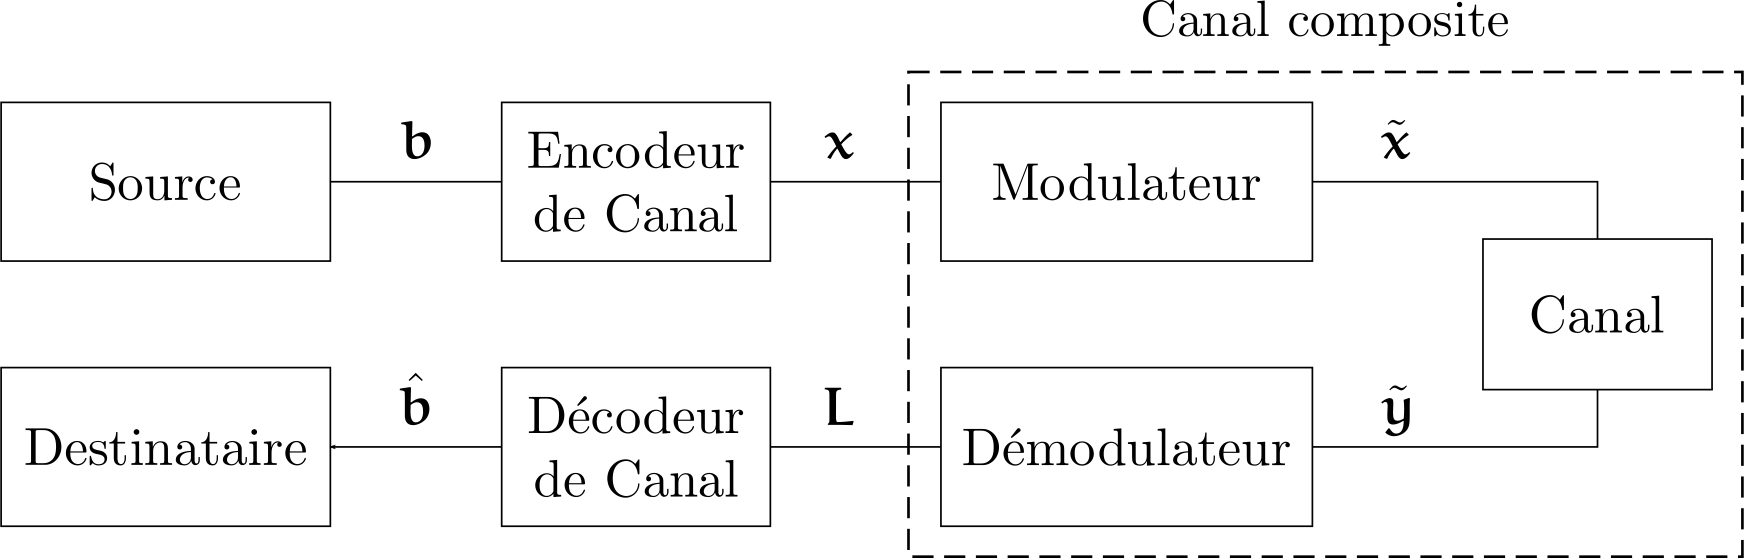
\includegraphics[width=0.8\textwidth]{main/ch1_fig/chaine_com}
\caption{Une chaîne de communication}
\label{fig:chaine_com}
\end{figure}
Une chaîne de communications numériques est représentée en Figure~\ref{fig:chaine_com}.
Elle représente les étapes usuelles de la transmission de données numériques depuis une \textbf{Source} vers un \textbf{Destinataire} à travers un \textbf{Canal}.
Le canal de transmission est le support qui permet le transfert de l'information. Lors de communications sans fil, il s'agit du vide, par lequel passent les ondes émises par les antennes de nos équipements. Or les grandeurs physiques associées à ce canal sont continues tandis que les données à transmettre sont une \textbf{séquence d'information} constituée de bits, donc discrètes. C'est le rôle du modulateur que de transformer ce flux binaire en signaux physiques transmissibles par le canal. Si l'on considère toujours le cas d'application des communications sans fils, le modulateur transforme des séquences de bits en formes d'ondes.

Au sein du canal de communication, les signaux subissent de nombreuses perturbations. Le bruit thermique des composants circuits électroniques de la chaine de transmission et les interférences causées par d'autres utilisateurs du canal sont des exemples de sources de perturbations. Le démodulateur, qui a le rôle inverse du modulateur, c'est-à-dire de convertir les signaux physiques en données binaires, peut, à cause de ces perturbations, commettre des erreurs. Ceci est un problème, puisque le but de la chaîne de transmission est de transmettre au destinataire l'exacte réplique de la séquence d'information donnée par la source. Dans le cas contraire, il s'agit d'erreurs de transmissions. La qualité de la chaine de transmission est souvent mesurée par son taux d'erreur binaire (BER), qui correspond au nombre de bits erronés sur le nombre total de bits transmis.

L'ajout d'un encodeur et d'un décodeur canal dans la chaîne de transmission est un moyen efficace de réduire ce taux d'erreur. L'encodeur transforme une séquence d'information $\mathbold{b}$ de $K$ bits en un \textbf{mot de code} $\mathbold{x}$ de $N$ bits. La taille du mot de code, en nombre de bits, est supérieure à la taille de la séquence d'informations afin d'ajouter de la redondance au message transmis: le rendement du code $R=K/N$ est inférieur à $1$. Cette redondance est utilisée par le décodeur canal, ou parfois le couple démodulateur - décodeur canal, afin de réduire le taux d'erreur binaire de la chaîne de transmission. Dans la présente thèse, le décodeur canal est découplé du démodulateur. L'ensemble modulateur - canal - démodulateur peut être considéré comme une entité indépendante dont l'entrée est le mot de code $\mathbold{x}$ et la sortie une séquence d'estimation $\mathbold{L}$. Cet ensemble est appelé canal composite.

\subsection{Le canal composite}
Un seul et unique modèle de canal composite sera considéré tout au long de ce manuscrit. Sa modulation est une modulation à changement de phase binaire (BPSK) qui associe aux valeurs binaires d'entrée $x\in\{0,1\}$ les valeurs réelles $\hat{x}\in\{-1,1\}$, respectivement.
Le canal à bruit blanc additif gaussien à double entrée (BI-AWGNC) tel que défini dans \cite[Section~1.5.1.3]{ryan2009channel} est considéré. Ce modèle est le plus utilisé pour caractériser les performances des codes correcteurs d'erreur car il se rapproche du bruit thermique évoqué précédemment, qui est souvent prépondérant. Il consiste en l'addition d'une variable réelle à distribution gaussienne centrée en $0$ et de densité spectrale $N_0$. Afin d'évaluer les performances de correction des codes correcteurs d'erreurs, les taux d'erreur seront souvent rapportés à cette densité spectrale, ou plus précisément au \textbf{rapport signal à bruit} (SNR), noté $E_b/N_0$, où $E_b=\frac{\mathbb{E}(\hat{x}^2)}{R}$ est l'énergie moyenne par bit d'information.

Les estimations en sortie du démodulateur sont données sous la forme de rapport de vraisemblance logarithmique (LLR). Leur signe détermine la valeur binaire d'entrée $x$ la plus probable, et leur valeur absolue le degré de fiabilité de cette valeur d'entrée. Des détails sur le modèle de canal et le calcul de ces LLRs sont données en Annexe \ref{append:canal}.

\subsection{Encodage de codes polaires}
Les codes polaires appartiennent à la famille des codes en blocs linéaire. Soient les ensembles $\mathbb{B}^n = \{0,1\}^n$, et  une matrice de taille $G \in \mathbb{B}^K \times \mathbb{B}^N$. L'encodage d'un code en blocs linéaire est une application linéaire injective de $\mathbb{B}^K$ vers $\mathbb{B}^N$ qui à un élément $\mathbold{b} \in \mathbb{B}^K$ associe un élément $\mathbold{x} \in \mathbb{B}^N$ tel que $x=bG$. Définir un encodeur de code polaire revient donc à définir sa matrice génératrice $G$. 

La matrice génératrice d'un code polaire est elle-même produit de deux matrices $E \in (\mathbb{B}^K \times \mathbb{B}^N)$ et $F^{\otimes n}\in (\mathbb{B}^N)^2$, $G=EF^{\otimes n}$. La multiplication par la matrice $E$ correspond à l'ajout de "bits gelés", dont la valeur est $0$, à la séquence d'information $\mb{b}$. Le résultat de l'opération $\mathbold{u} = E\mathbold{b}$ est constitué de $K$ bits $b_i \in \mathbold{b}$ et de $N-K$ bits gelés. Les positions respectives des bits d'informations et des bits gelés sont liés au phénomène de polarisation décrit dans la section suivante est sont déterminants quant à la performance de correction du code.

La matrice $F^{\otimes n}$, où $N=2^n$, est la n-ième puissance de Kronecker du noyau $F=\left[\begin{smallmatrix} 1 & 0 \\ 1 & 1\end{smallmatrix}\right]$. En Figure \ref{fig:encodage} sont données plusieurs représentations de cette matrice d'encodage. La représentation sous forme de \textit{factor graph} est une représentation alternative où les symboles $\oplus$ correspondent à des opération \textit{OU-exclusif}. La représentation sous forme d'arbre binaire est quant à elle particulièrement pertinente pour la description des algorithmes de décodage.

\begin{figure}[t]
\centering
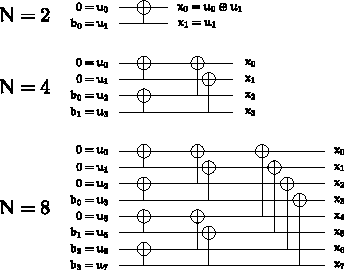
\includegraphics[width=0.7\textwidth]{main/ch1_fig/Graph_N_rec}
\caption{Différentes représentation de l'encodage de codes polaires}
\label{fig:encodage}
\end{figure}

Le processus d'encodage peut également être modifié pour rendre le code systématique. Un code correcteur d'erreur est dit systématique si les bits de la séquence d'information sont présents dans le mot de code. Pour se faire, il faut modifier la matrice d'encodage : $G_{sys}=EF^{\otimes n}EF^{\otimes n}$. Il est alors prouvé dans \cite{arikan_systematic_2011} que si $\mb{x}=\mb{b}G_{sys}$, alors $\mb{b}=E^{-1}\mb{x}$. L'encodage systématique est représenté en Figure \ref{fig:sys}.

\begin{figure}[t]
\centering
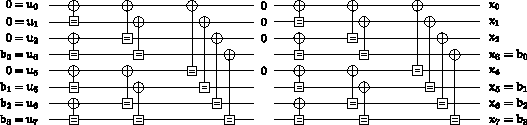
\includegraphics[width=0.7\textwidth]{main/ch1_fig/Graph_N_sys}
\caption{Encodage systématique}
\label{fig:sys}
\end{figure}

\subsection{Polarisation}

L'invention des codes polaires et la définition des matrices d'encodage par Ar{\i}kan \cite{arikan_channel_2009} est lié au phénomène de polarisation. L'ensemble constitué de l'encodeur polaire, du canal composite et du décodeur polaire peut être vu comme un ensemble de canaux de transmission qui chacun transmet un bit. On parle de polarisation parce que, dans ces condition, il est possible de montrer que ces $N$ canaux ont tendance à se diviser en deux groupes. Un groupe de canaux très fiables, avec une probabilité d'erreur faible, et un groupe de canaux peu fiables, à probabilité d'erreur forte. Cette tendance augmente quand $N$ augmente, les canaux se polarisent. Ainsi, les bits d'informations seront attribués aux canaux fiables, et des bits dits gelés, dont la valeur est connue à priori, seront attribués aux canaux peu fiables. Le processus de détermination de la position des bits gelés dans le vecteur $\mathbold{u}$ est appelé construction des codes polaires. Celle-ci est déterminante pour la performance de correction des codes polaires. Plusieurs méthodes efficaces ont été proposées \cite{tal_how_2013,trifonov_efficient_2012} pour le canal AWGN.

\section{Les algorithmes de décodage de codes polaires}

Deux algorithmes de décodages ont été proposés dès l'invention des codes polaires \cite{arikan_channel_2009}. L'algorithme de décodage appelé Annulation Successive (SC) est un algorithme de décodage à sortie dure : les données de sortie sont des bits. L'algorithme de décodage par propagation de croyance (BP) est au contraire un algorithme de décodage à sortie souple, dont les données de sortie sont des estimations représentée par exemple par des LLRs. De nombreuses variantes de ces algorithme ont ensuite été proposées pour améliorer leur performances de corrections. Les algorithme Annulation Successive par Liste (SCL), Annulation Successive "Flip" (SCF), Annulation Sucessive par Pile (SCS) sont des évolutions de l'algorithme SC. Tandis que l'algorithme appelé Annulation Souple (SCAN) eut être vu comme une combinaison des algorithmes SC et BP. Chacun de ces algorithmes est décrit dans cette section.

\subsection{Annulation Successive}
\begin{figure}[t]
\centering
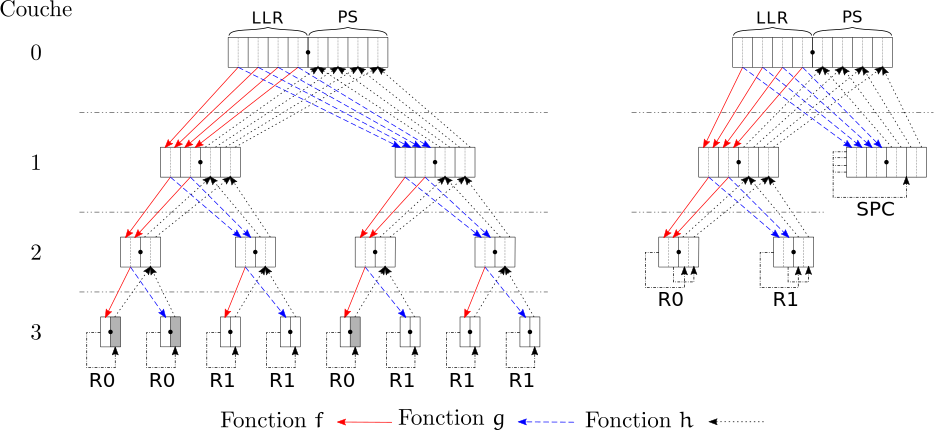
\includegraphics[width=0.7\textwidth]{main/ch1_fig/sc}
\caption{Arbre de décodage SC}
\label{fig:sc}
\end{figure}
% Sommes partielles termes non introduit
% Vérifier que n est introduit
Les données d'entrée des algorithmes de décodages présentés ici sont des LLRs, contenus dans le vecteur $\mathbold{L}$ de taille $N$, sortis du canal composite. Les données de sorties sont des bits contenus dans le vecteur $\mathbold{\hat{b}}$ de taille $K$. Au cours du décodage de codes polaires, ces deux formats de données (LLRs et bits) sont également utilisés. La Figure~\ref{fig:sc} représente ces données nécessaires. Dans l'exemple considéré, $K=3$ et $N=8$. Les données sont organisées en arbre binaire sur $log_2(N) + 1$ couches. Dans notre cas donc, l'arbre possède quatre niveaux. A chaque couche sont attribués un certain nombre de noeuds. La racine de l'arbre numérotée $0$ est constituée d'un seul noeud. Ce noeud contient $N$ LLRs et $N$ sommes partielles. En decendant dans l'arbre, à chaque couche, le nombre de noeuds double, tandis que le nombre de LLRs et de sommes partielles de chaque noeud et divisé par deux. Chaque couche $d$ contient $2^d$ noeuds constitués de $2^{n-d}$ LLRs et de $2^{n-d}$ sommes partielles. 

% Ajouter channel LLRs à la racine

La première étape du décodage est le chargement des LLRs du canal $L$ : les LLRs du noeud racine prennent la valeur des LLRs du canal. Les LLRs et les sommes partielles de chaque noeud de l'arbre sont ensuite calculées par l'intermédiaire des opérations $f$, $g$, $h$, \texttt{R0} et \texttt{R1} symbolisées dans la Figure~\ref{fig:sc} par des flèches. Elles correspondent aux équations \ref{eq:sc}. 
    \begin{eqnarray}
      \begin{array}{l c l}
        f(L_a,L_b) &=& \text{sign}(L_a.L_b).\min(|L_a|,|L_b|)\\
        g(L_a,L_b,\hat{s}_a)&=&(1-2\hat{s}_a)L_a+L_b\\
        h(\hat{s}_a,\hat{s}_b)&=& (\hat{s}_{a} \oplus \hat{s}_{b}, \hat{s}_{b})\\
        \texttt{R0}(L_a) &=& 0 \\
        \texttt{R1}(L_a) &=&  \left\{\begin{array}{l c l} 0 \text{ si } L_a \geq 0 \\ 1 \text{ si } L_a < 0 \end{array}\right.
      \end{array}
      \label{eq:sc}
    \end{eqnarray}
% Explixiter notation (N,K)
Les fonctions $f$ et $g$ prennent comme entrée des LLRs et produisent des LLRs en sortie. Elles permettent de descendre dans l'arbre jusqu'aux feuilles. Les feuilles sont les noeuds les plus bas de l'arbre. Le traitement d'une feuille correspond à l'application des opérations \texttt{R0} et \texttt{R1}. Lors d'un décodage non systématique, les sommes partielles contenues par les feuilles correspondent aux bits du mot de code. Certains sont donc des bits d'informations, d'autres sont des bits gelés dont la valeur, $0$, est connue d'avance. Pour les feuilles contenant les bits gelés, l'opération \texttt{R0} est appliquée, la somme partielle est égale à 0. Lorsque la feuille contient un bit d'information, l'opération \texttt{R1} est appliquée, la somme partielle est obtenue par seuillage du LLR. Après le décodage d'une feuille, la fonction $h$ est appliquée afin de remonter dans l'arbre. La hauteur jusqu'à laquelle les sommes partielles sont calculées grâce à la fonction $h$ dépend de l'index de la feuille qui vient d'être décodé. Cette recombinaison des sommes partielles est nécessaire à l'application des fonctions $g$, qui prennent en argument des sommes partielles. Le séquencement du décodage SC d'un codes polaire de taille $N=4$ est détaillé en Figure~\ref{fig:seq_sc}.

\begin{figure}[b]
\centering
\includegraphics[width=0.5\textwidth]{main/ch1_fig/seq_sc}
\caption{Séquencement du décodage SC d'un code polaire de taille $N=8$.}
\label{fig:seq_sc}
\end{figure}

\begin{itemize}
\item Parallélisme
\item Systématique
\end{itemize}
\subsection{Annulation Successive Liste}
\begin{itemize}
\item Algorithme
\item Calcul Métrique

\end{itemize}
\subsection{Algorithmes itératifs à sortie souple}
\begin{itemize}
\item Noeud 2 à sortie souple
\item BP
\item SCAN
\end{itemize}

\subsection{Autres algorithmes}
\begin{itemize}
	\item SCS
	\item SCF
\end{itemize}
\section{Améliorations algorithmiques}

\subsection{Elagage de l'arbre de décodage}

\subsubsection{Fast SC}
\begin{itemize}
\item R0 - R1
\item SPC - REP
\item détailler calculs évitables (g0, f0, grep)
\end{itemize}
\subsubsection{Fast SCL}
\begin{itemize}
\item détailler adaptation élagage pour SC Liste - calculs métriques
\item discussion chase spc - r1 ? Hashemi-Sarkis + Simulations
\end{itemize}
\subsubsection{Fast SCAN}
\begin{itemize}
\item 
\end{itemize}

\subsection{Adaptive}

\section{Codes polaires de taille variables}
% https://arxiv.org/pdf/1701.06458.pdf 4-5-6-7-8-9


\subsection*{Conclusion}
